% ─────────────────────────────────────────────────────────────────────────────
%
% Documentación de la alineación gravitacional a la nube de puntos.
% ─────────────────────────────────────────────────────────────────────────────

\section{Alineación gravitacional de la nube de puntos}
\label{sec:lm-gravity-aligner}

La primera iteración del módulo (sección~\ref{sec:lm-depth-projector})
produce una nube de puntos 3D en el frame óptico de la cámara. Dicho frame
no está alineado con el mundo físico: si la cámara se encuentra inclinada
respecto del plano horizontal, el suelo no aparece como un plano horizontal
en la nube, y los objetos verticales no son paralelos al eje que representa
la verticalidad. Esta iteración introduce la corrección de esa inclinación
mediante el uso del acelerómetro integrado en el sensor.

\subsection{Marco teórico}

\subsubsection{Estimación de orientación estática por acelerómetro}

En condiciones cuasi-estáticas (usuario en reposo o en movimiento lento), la
aceleración medida por el acelerómetro corresponde casi exclusivamente a la
aceleración gravitacional. El vector de aceleración medido $\mathbf{a}_s$,
expresado en el frame del sensor, apunta en la dirección opuesta a la
gravedad tal como la observa el sensor. Esta propiedad permite estimar la
inclinación relativa entre el sensor y el plano horizontal del mundo sin
necesidad de un sistema de referencia externo.

En el frame óptico de la cámara (convención RealSense D435), los ejes son:
\begin{itemize}
  \item $x$: apunta hacia la derecha.
  \item $y$: apunta hacia abajo.
  \item $z$: apunta hacia adelante (hacia la escena).
\end{itemize}
Cuando la cámara está perfectamente horizontal, el acelerómetro mide
$\mathbf{a}_s = (0,\, -g,\, 0)$, donde $g \approx 9{,}81\,\text{m/s}^2$,
como se ilustra en la Figura~\ref{fig:cam-horizontal}.
El signo negativo se debe a que el acelerómetro registra la reacción de la
estructura del sensor ante la gravedad: en ausencia de aceleración externa,
la fuerza aparente experimentada por el sensor es igual y opuesta al vector
gravitacional. Cualquier desviación respecto de ese valor indica una
inclinación de la cámara.

\begin{figure}[ht]
  \centering
  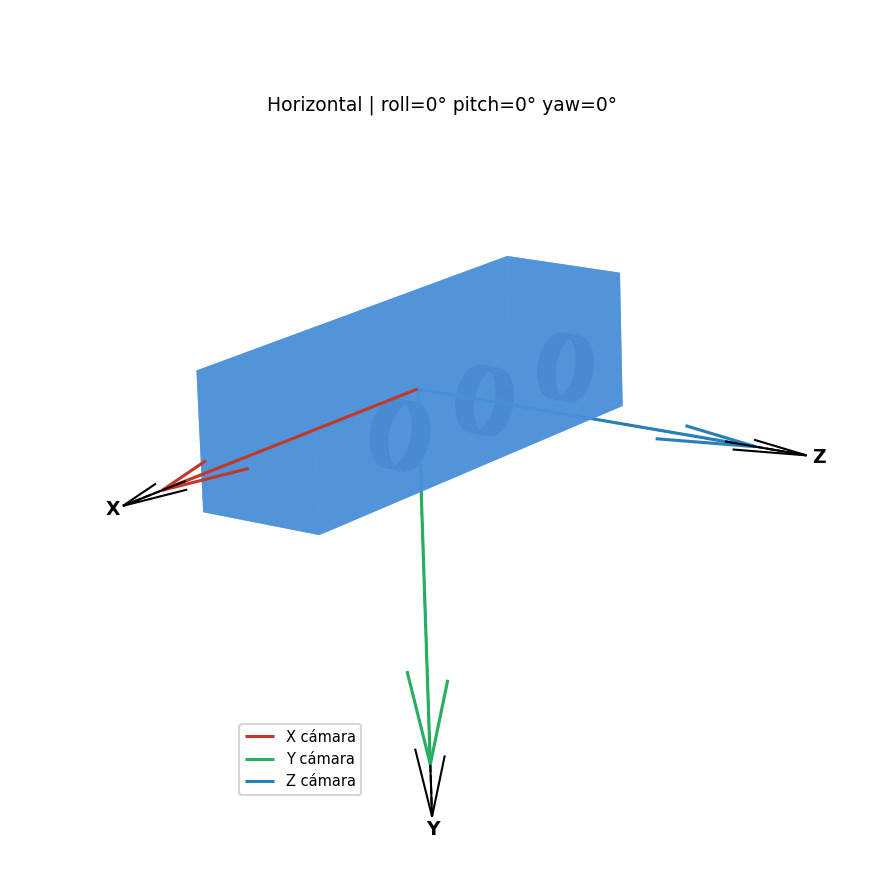
\includegraphics[width=0.45\textwidth]{_Imagenes/local_mapper/horizontal.png}
  \caption{Cámara D435i en posición horizontal. El acelerómetro mide
           $(0,\,-g,\,0)$ y no se requiere corrección alguna.}
  \label{fig:cam-horizontal}
\end{figure}

\subsubsection{Ángulos de Euler y sus limitaciones}

Una forma intuitiva de representar la inclinación de la cámara es mediante
los ángulos de Euler: \emph{roll} ($\phi$), \emph{pitch} ($\theta$) y
\emph{yaw} ($\psi$), que describen tres rotaciones sucesivas alrededor de
ejes fijos. En la convención de la cámara ($x$ derecha, $y$ abajo, $z$
adelante), roll es la rotación alrededor de $z$ (inclinación lateral), pitch
es la rotación alrededor de $x$ (inclinación hacia adelante o atrás) y yaw
es la rotación alrededor de $y$ (giro sobre el eje vertical), tal como se
ilustra en la Figura~\ref{fig:euler-angles}.

\begin{figure}[ht]
  \centering
  \begin{minipage}[b]{0.32\textwidth}
    \centering
    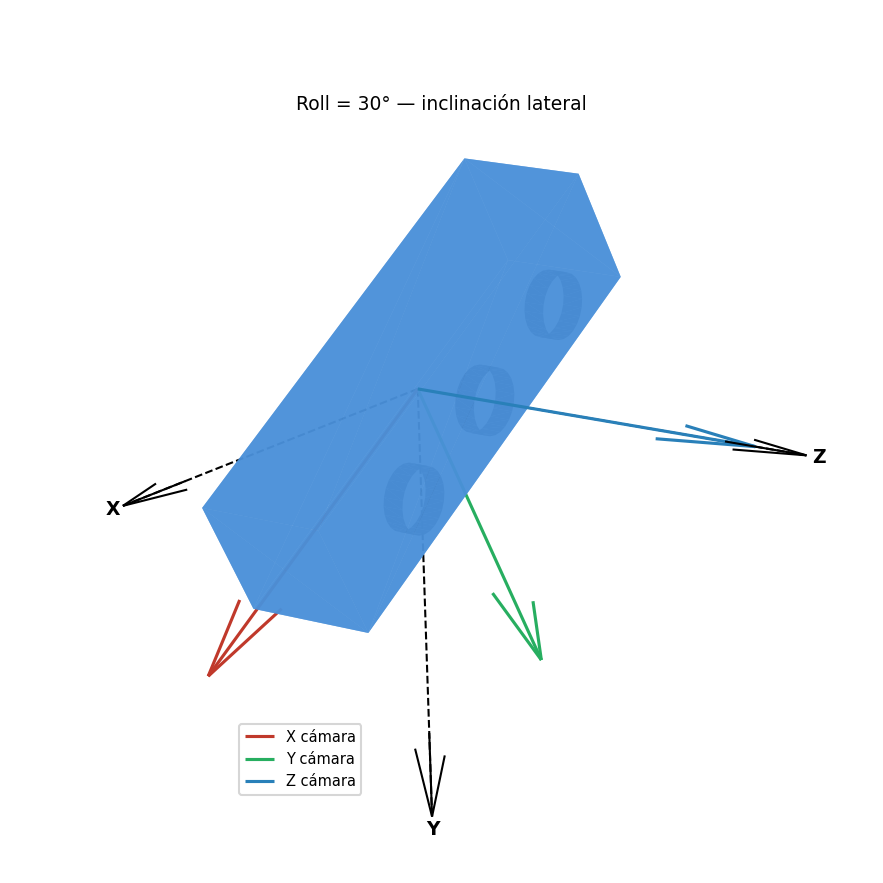
\includegraphics[width=\textwidth]{_Imagenes/local_mapper/roll_30.png}
    \subcaption{Roll $= 30°$: rotación \\ alrededor de $z$.}
    \label{fig:cam-roll-30}
  \end{minipage}
  \hfill
  \begin{minipage}[b]{0.32\textwidth}
    \centering
    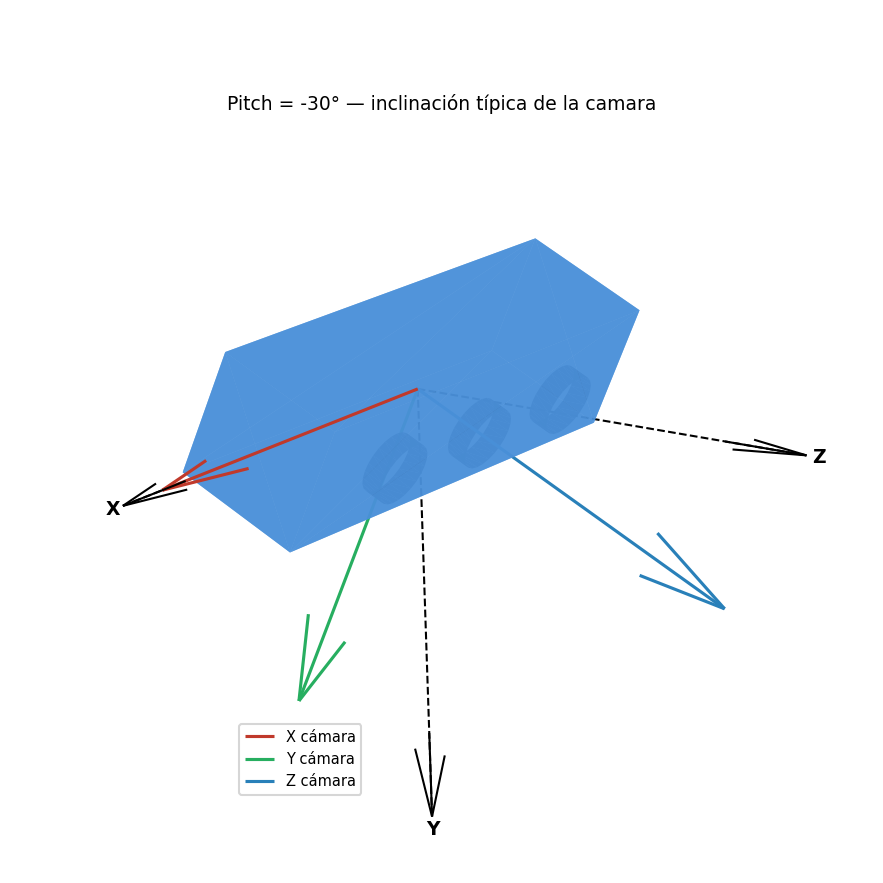
\includegraphics[width=\textwidth]{_Imagenes/local_mapper/pitch_n30.png}
    \subcaption{Pitch $= -30°$: rotación \\ alrededor de $x$.}
    \label{fig:cam-pitch-30}
  \end{minipage}
  \hfill
  \begin{minipage}[b]{0.32\textwidth}
    \centering
    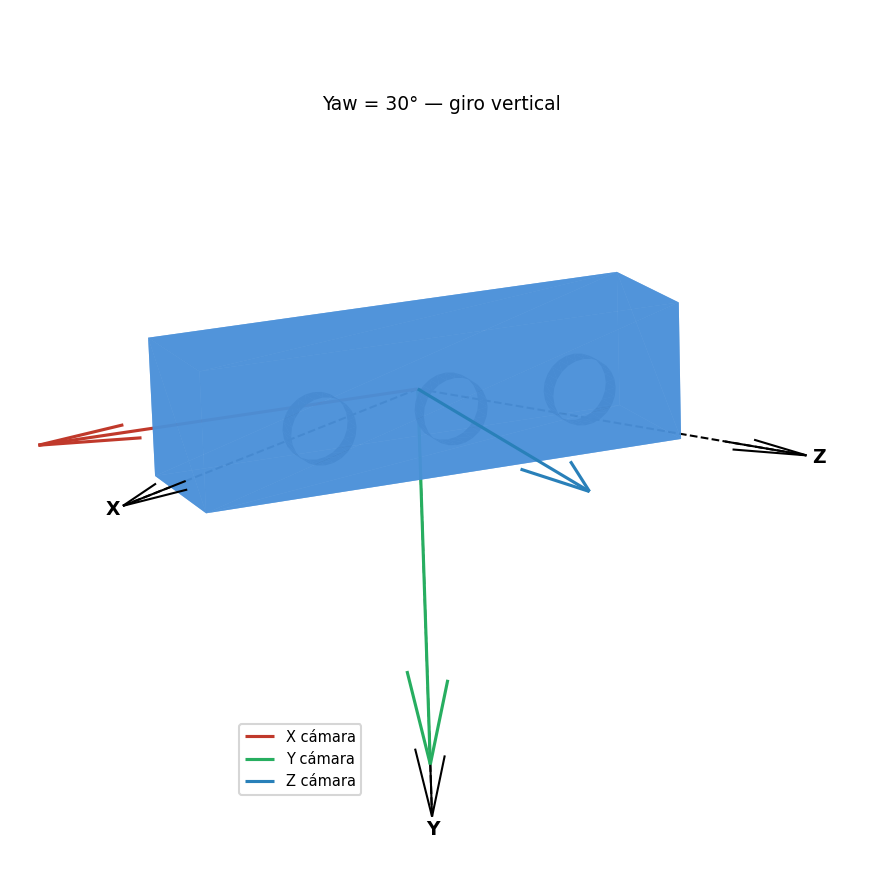
\includegraphics[width=\textwidth]{_Imagenes/local_mapper/yaw_30.png}
    \subcaption{Yaw $= 30°$: rotación \\ alrededor de $y$.}
    \label{fig:cam-yaw-30}
  \end{minipage}
  \caption{Los tres ángulos de Euler en la convención del frame óptico de la
           cámara. Cada rotación se realiza alrededor de un eje fijo del
           sensor: $z$ (roll), $x$ (pitch) e $y$ (yaw).}
  \label{fig:euler-angles}
\end{figure}

A partir de la lectura del acelerómetro se pueden estimar roll y pitch
directamente mediante las ecuaciones~\ref{eq:roll} y~\ref{eq:pitch}:
\begin{align}
  \phi    &= \arctan\!\left(\frac{a_x}{a_y}\right) \label{eq:roll} \\
  \theta  &= \arctan\!\left(\frac{a_z}{\sqrt{a_x^2 + a_y^2}}\right) \label{eq:pitch}
\end{align}
El ángulo de yaw ($\psi$) no puede obtenerse del acelerómetro porque este
mide únicamente la dirección del vector gravitacional, que es paralela al eje
$y$. Una rotación pura alrededor de $y$ (yaw) no modifica la proyección del
vector gravitacional sobre ningún eje del sensor, por lo que dicha rotación
es invisible para el acelerómetro.

Sin embargo, incluso limitándose a roll y pitch, la representación por
ángulos de Euler presenta una singularidad conocida como \emph{gimbal lock}.
Cuando $\theta = \pm 90°$, la cámara apunta verticalmente y el eje de roll
($z$, que en posición nominal apunta hacia adelante) queda alineado con el
eje de yaw ($y$, que apunta hacia abajo en el mundo). En esa configuración,
girar roll o girar yaw produce exactamente el mismo efecto sobre la
orientación del sensor: el sistema dispone de dos grados de libertad para
describir el mismo movimiento y pierde uno de los tres originales, haciendo
que la representación se vuelva indefinida. Este escenario es alcanzable en
el equipo final cuando el usuario inclina la cabeza pronunciadamente hacia adelante,
llevando la cámara a apuntar verticalmente hacia abajo (pitch $= -90°$).
La formulación mediante cuaterniones evita este problema de manera elegante
y sin costo adicional, como se desarrolla en la sección siguiente.
La Figura~\ref{fig:cam-gimbal} ilustra esta configuración crítica.

Este problema no es meramente teórico. Durante el programa Apollo, la unidad
de medición inercial (IMU) utilizaba tres gimbals mecánicos para mantener
una plataforma estabilizada independientemente de la actitud de la nave.
Los ingenieros del MIT decidieron conscientemente no incorporar un cuarto
gimbal: en cambio, el computador de guiado emitía una advertencia al superar
los $70°$ de inclinación y congelaba la plataforma en la singularidad al
alcanzar los $85°$, requiriendo realineación manual mediante
estrellas~\cite{Hoag1963,Jones2006Gimbals}. La solución moderna, adoptada
en este trabajo, consiste en montar los sensores directamente sobre el cuerpo
del dispositivo (\emph{strapdown}) e integrar digitalmente las rotaciones
mediante cuaterniones, eliminando el problema de forma estructural.

\begin{figure}[ht]
  \centering
  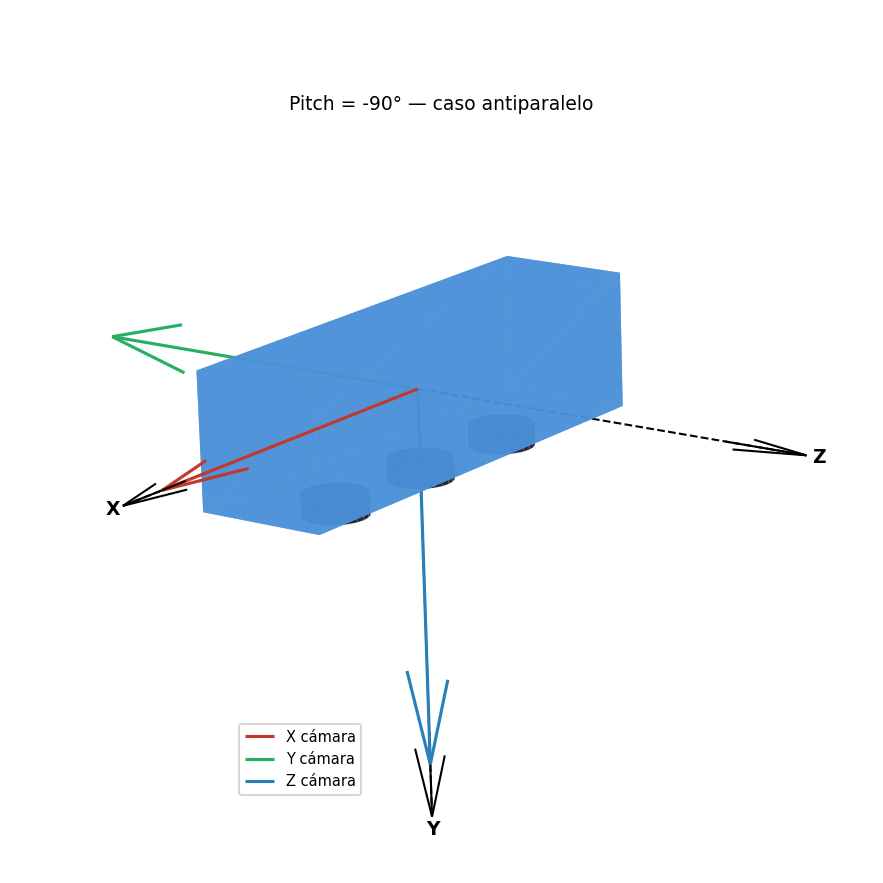
\includegraphics[width=0.45\textwidth]{_Imagenes/local_mapper/pitch_n90.png}
  \caption{Singularidad \emph{gimbal lock}: con pitch $= -90°$ la cámara apunta
           verticalmente hacia abajo, el eje de roll ($z$) queda alineado con el
           eje de yaw ($y$) y la representación por ángulos de Euler se vuelve
           indefinida. Esta orientación es alcanzable en el equipo final ante
           una inclinación pronunciada de la cabeza del usuario hacia adelante.}
  \label{fig:cam-gimbal}
\end{figure}

\subsubsection{Cuaterniones y rotación en 3D}

Un cuaternión es una extensión de los números complejos al espacio
tridimensional, propuesta por Hamilton en 1843. Se define como se muestra
en la ecuación~\ref{eq:quat-def}:
\begin{equation}
  \label{eq:quat-def}
  q = q_w + q_x\,\mathbf{i} + q_y\,\mathbf{j} + q_z\,\mathbf{k}
\end{equation}
donde $q_w \in \mathbb{R}$ es la parte escalar y
$\mathbf{q}_v = (q_x, q_y, q_z)^T$ es la parte vectorial, con
$\mathbf{i}, \mathbf{j}, \mathbf{k}$ las unidades imaginarias que satisfacen
$\mathbf{i}^2 = \mathbf{j}^2 = \mathbf{k}^2 = \mathbf{i}\mathbf{j}\mathbf{k} = -1$.
Se escribe de forma compacta como $q = (q_w,\, \mathbf{q}_v)$.

Un cuaternión unitario ($\|q\| = 1$) puede representar una rotación de
ángulo $\theta$ alrededor de un eje unitario $\hat{\mathbf{n}}$ como se
indica en la ecuación~\ref{eq:quat-unit}:
\begin{equation}
  \label{eq:quat-unit}
  q = \left(\cos\frac{\theta}{2},\; \hat{\mathbf{n}}\sin\frac{\theta}{2}\right)
\end{equation}
Su conjugado es $q^* = (q_w,\, -\mathbf{q}_v)$, que representa la rotación
inversa.

Un \emph{cuaternión puro} es aquel con parte escalar nula: $q_p = (0, \mathbf{p})$.
Se usa para representar puntos o vectores tridimensionales dentro del álgebra
de cuaterniones. La rotación de un vector $\mathbf{p}$ por el cuaternión
unitario $q$ se expresa mediante el producto triple de la
ecuación~\ref{eq:quat-rotation}:
\begin{equation}
  \label{eq:quat-rotation}
  \mathbf{p}' = q \otimes (0,\,\mathbf{p}) \otimes q^*
\end{equation}
donde $\otimes$ denota el producto de Hamilton. Dado $q = (q_w,\, q_x,\, q_y,\, q_z)$
y el cuaternión puro $p = (0,\, p_x,\, p_y,\, p_z)$, el producto se computa
en dos pasos. En el primero se obtiene el cuaternión intermedio
$t = q \otimes p$, cuyos componentes son los de la
ecuación~\ref{eq:hamilton-qp}:
\begin{equation}
  \label{eq:hamilton-qp}
  t = \begin{pmatrix} t_w \\ t_x \\ t_y \\ t_z \end{pmatrix}
    = \begin{pmatrix}
        -q_x p_x - q_y p_y - q_z p_z \\
         q_w p_x + q_y p_z - q_z p_y \\
         q_w p_y + q_z p_x - q_x p_z \\
         q_w p_z + q_x p_y - q_y p_x
      \end{pmatrix}
\end{equation}
En el segundo paso se multiplica por $q^* = (q_w,\, -q_x,\, -q_y,\, -q_z)$, y
la parte vectorial del resultado, que constituye el vector rotado
$\mathbf{p}'$, es la de la ecuación~\ref{eq:hamilton-tqc}:
\begin{equation}
  \label{eq:hamilton-tqc}
  \mathbf{p}' = \begin{pmatrix} p'_x \\ p'_y \\ p'_z \end{pmatrix}
    = \begin{pmatrix}
        -t_w q_x + t_x q_w - t_y q_z + t_z q_y \\
        -t_w q_y + t_x q_z + t_y q_w - t_z q_x \\
        -t_w q_z - t_x q_y + t_y q_x + t_z q_w
      \end{pmatrix}
\end{equation}
Esta expansión es equivalente a aplicar una matriz de rotación
$R \in SO(3)$, pero numéricamente más estable y eficiente al componer
múltiples rotaciones. La Figura~\ref{fig:quat-orientations} ilustra dos
ventajas concretas de esta representación: la composición natural de
rotaciones y la representación unívoca de orientaciones que los ángulos de
Euler no pueden distinguir en la singularidad.

\begin{figure}[ht]
  \centering
  \begin{minipage}[b]{0.48\textwidth}
    \centering
    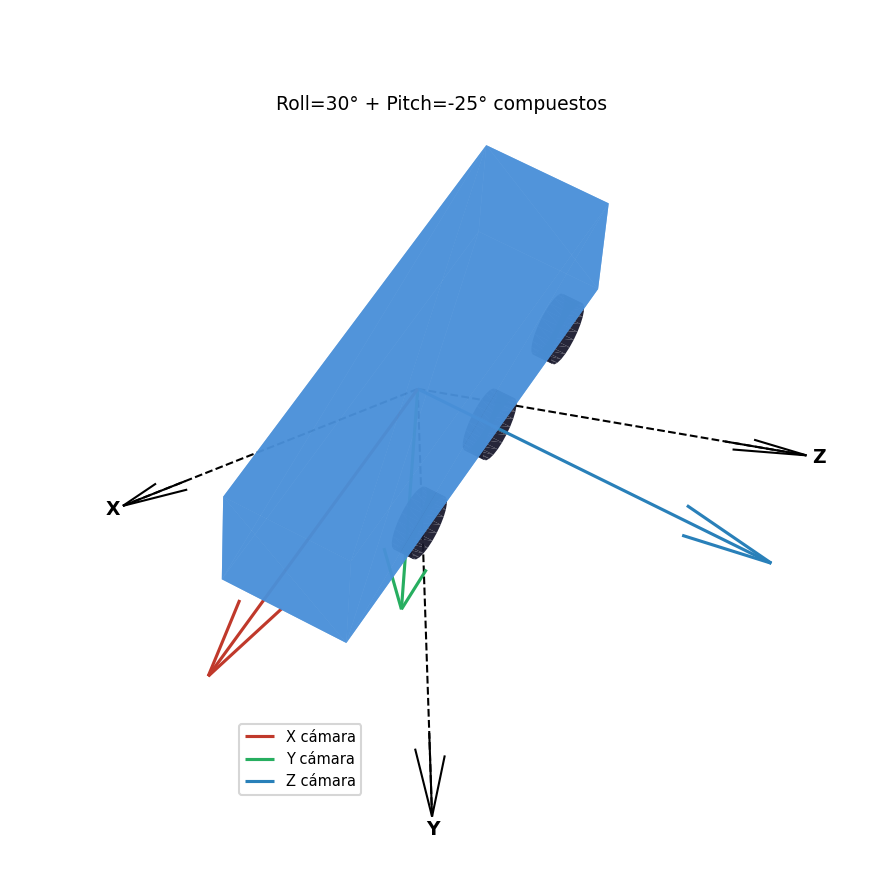
\includegraphics[width=\textwidth]{_Imagenes/local_mapper/roll30_pitch_n25.png}
    \subcaption{Roll $= 30°$ y pitch $= -25°$ compuestos. \\
                $q = (0{,}943,\; -0{,}209,\; -0{,}056,\; 0{,}253)$.}
    \label{fig:cam-quat-composed}
  \end{minipage}
  \hfill
  \begin{minipage}[b]{0.48\textwidth}
    \centering
    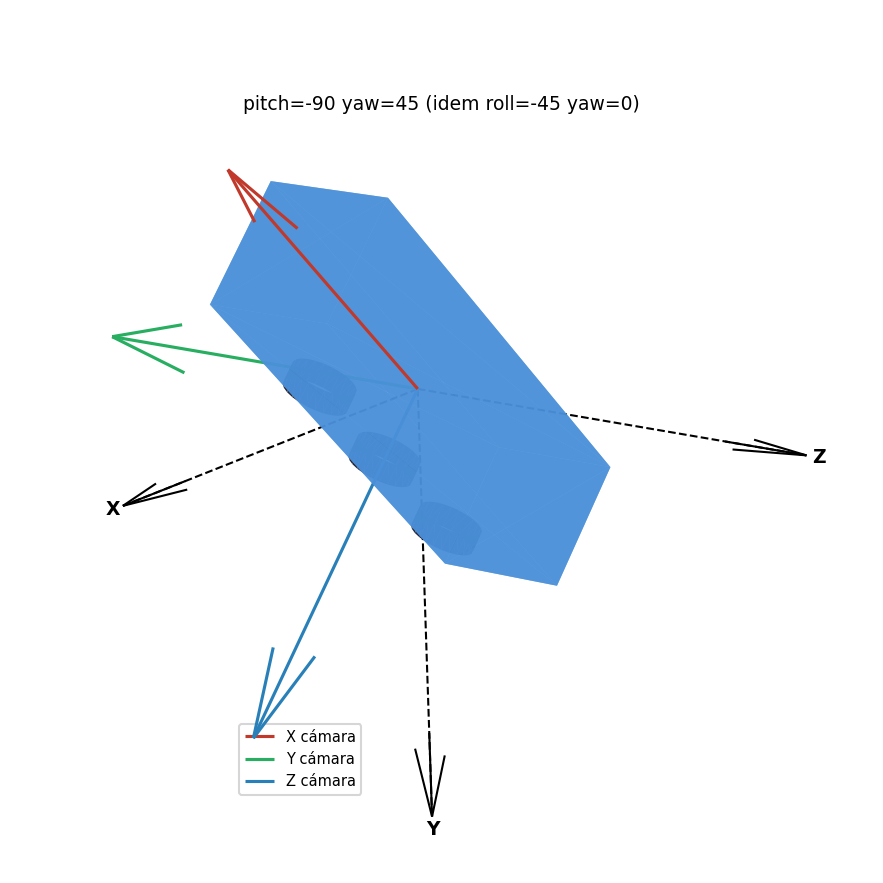
\includegraphics[width=\textwidth]{_Imagenes/local_mapper/gimbal_lock_ambiguous.png}
    \subcaption{Pitch $= -90°$, yaw $= 45°$: orientación en la singularidad. \\
                $q = (0{,}653,\; -0{,}653,\; 0{,}271,\; -0{,}271)$.}
    \label{fig:cam-quat-gimbal-ambiguous}
  \end{minipage}
  \caption{Ventajas de la representación mediante cuaterniones. A la izquierda,
           una rotación compuesta (roll y pitch simultáneos) se codifica en un
           único cuaternión unitario sin ambigüedad de orden. A la derecha, una
           orientación en la singularidad de gimbal lock (pitch $= -90°$):
           las ternas $(\phi=0°,\,\theta=-90°,\,\psi=45°)$ y
           $(\phi=-45°,\,\theta=-90°,\,\psi=0°)$ producen exactamente la misma
           orientación física y el mismo cuaternión, evidenciando que los ángulos
           de Euler pierden un grado de libertad mientras que el cuaternión la
           representa de forma unívoca.}
  \label{fig:quat-orientations}
\end{figure}

\subsubsection{Rotación mínima entre dos vectores}

El problema concreto consiste en encontrar el cuaternión $q$ que rota el
vector de aceleración normalizado $\hat{\mathbf{a}}$ hasta coincidir con el
vector ``abajo'' canónico $\hat{\mathbf{b}} = (0, -1, 0)$. La rotación
mínima (geodésica en $SO(3)$) entre dos vectores unitarios
$\hat{\mathbf{a}}$ y $\hat{\mathbf{b}}$ tiene:
\begin{itemize}
  \item eje de rotación: $\hat{\mathbf{n}} = \hat{\mathbf{a}} \times \hat{\mathbf{b}}$
        (perpendicular a ambos vectores).
  \item ángulo de rotación: $\theta = \arccos(\hat{\mathbf{a}} \cdot \hat{\mathbf{b}})$.
\end{itemize}
En lugar de calcular explícitamente $\hat{\mathbf{n}}$ y $\theta$, se construye
el cuaternión en forma proporcional y se normaliza al final. Sustituyendo
$\hat{\mathbf{n}} = (\hat{\mathbf{a}} \times \hat{\mathbf{b}})/\sin\theta$
y $\cos\theta = \hat{\mathbf{a}} \cdot \hat{\mathbf{b}}$ en la
ecuación~\ref{eq:quat-unit}:
\begin{equation}
  q = \left(\cos\frac{\theta}{2},\;
      \frac{\hat{\mathbf{a}} \times \hat{\mathbf{b}}}{\sin\theta}\,
      \sin\frac{\theta}{2}\right)
  = \left(\cos\frac{\theta}{2},\;
      \frac{\hat{\mathbf{a}} \times \hat{\mathbf{b}}}{2\cos(\theta/2)}\right)
\end{equation}
donde se usó la identidad $\sin\theta = 2\sin(\theta/2)\cos(\theta/2)$.
Multiplicando ambas componentes por $2\cos(\theta/2)$ (escalar positivo que
no afecta la dirección del cuaternión) y aplicando
$2\cos^2(\theta/2) = 1 + \cos\theta = 1 + \hat{\mathbf{a}} \cdot \hat{\mathbf{b}}$,
se obtiene el cuaternión proporcional de las ecuaciones~\ref{eq:qmin-w}
y~\ref{eq:qmin-v}:
\begin{align}
  q_w        &= 1 + \hat{\mathbf{a}} \cdot \hat{\mathbf{b}} \label{eq:qmin-w}\\
  \mathbf{q}_v &= \hat{\mathbf{a}} \times \hat{\mathbf{b}}  \label{eq:qmin-v}
\end{align}
seguida de la normalización $q \leftarrow q / \|q\|$. En el caso particular
donde $\hat{\mathbf{b}} = (0, -1, 0)$, el producto escalar es
$\hat{\mathbf{a}} \cdot \hat{\mathbf{b}} = -a_y$ y el producto vectorial es
$\hat{\mathbf{a}} \times \hat{\mathbf{b}} = (a_z,\; 0,\; -a_x)$,
por lo que las expresiones se simplifican a la ecuación~\ref{eq:qmin-simplified}:
\begin{equation}
  \label{eq:qmin-simplified}
  q_w = 1 - a_y, \qquad
  \mathbf{q}_v = (a_z,\; 0,\; -a_x)
\end{equation}
donde $(a_x, a_y, a_z)$ es la aceleración normalizada.

Existe un caso degenerado que requiere tratamiento especial: cuando
$\hat{\mathbf{a}} = (0,+1,0)$, es decir $\hat{\mathbf{a}} \cdot \hat{\mathbf{b}} = -1$.
Esto ocurre cuando el eje $y$ del sensor queda apuntando hacia arriba en el
mundo, condición que se produce si la cámara gira $180°$ alrededor de $x$
(pitch $= 180°$): el lente pasa a apuntar hacia atrás y el lado superior
de la cámara queda orientado hacia el cielo. Este escenario es más factible
que otras inversiones, ya que podría ocurrir si el usuario inclina la cabeza
completamente hacia adelante llevando la cámara montada más allá de la
vertical. En esa situación existen infinitos ejes perpendiculares a $y$
alrededor de los cuales una rotación de $180°$ lleva $\hat{\mathbf{a}}$ a
$\hat{\mathbf{b}}$: el producto vectorial $\hat{\mathbf{a}} \times \hat{\mathbf{b}}$
se anula y el algoritmo no puede determinar el eje automáticamente. Se adopta
una rotación de $180°$ alrededor del eje $x$ como convenio, coherente con la
perturbación que originó el caso, resultando en $q = (0,\, 1,\, 0,\, 0)$.

Cabe destacar que esta ambigüedad en la elección del eje es distinta al
gimbal lock descrito en la sección anterior. El gimbal lock es una
singularidad de la \emph{representación} por ángulos de Euler que los
cuaterniones evitan completamente; la ambigüedad aquí es puramente geométrica
e inherente al problema de rotar $180°$ entre dos vectores antiparalelos,
independientemente de la representación utilizada. En cualquier caso, esta
situación (cámara apuntando exactamente hacia arriba) es prácticamente
inalcanzable en el dispositivo final. Estos casos límite se ilustran en la
Figura~\ref{fig:rot-min-cases}.

\begin{figure}[ht]
  \centering
  \begin{minipage}[b]{0.48\textwidth}
    \centering
    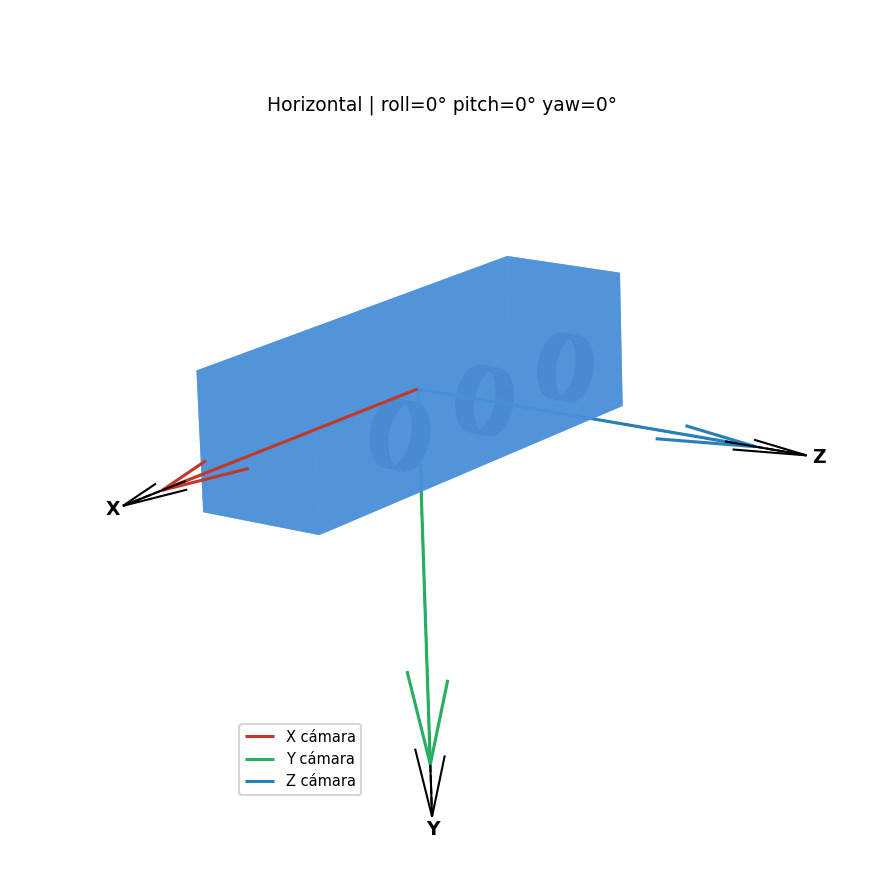
\includegraphics[width=\textwidth]{_Imagenes/local_mapper/horizontal.png}
    \subcaption{Horizontal: $\hat{\mathbf{a}} = (0,-1,0) = \hat{\mathbf{b}}$. \\
                El cuaternión calculado es la identidad.}
    \label{fig:rot-min-identity}
  \end{minipage}
  \hfill
  \begin{minipage}[b]{0.48\textwidth}
    \centering
    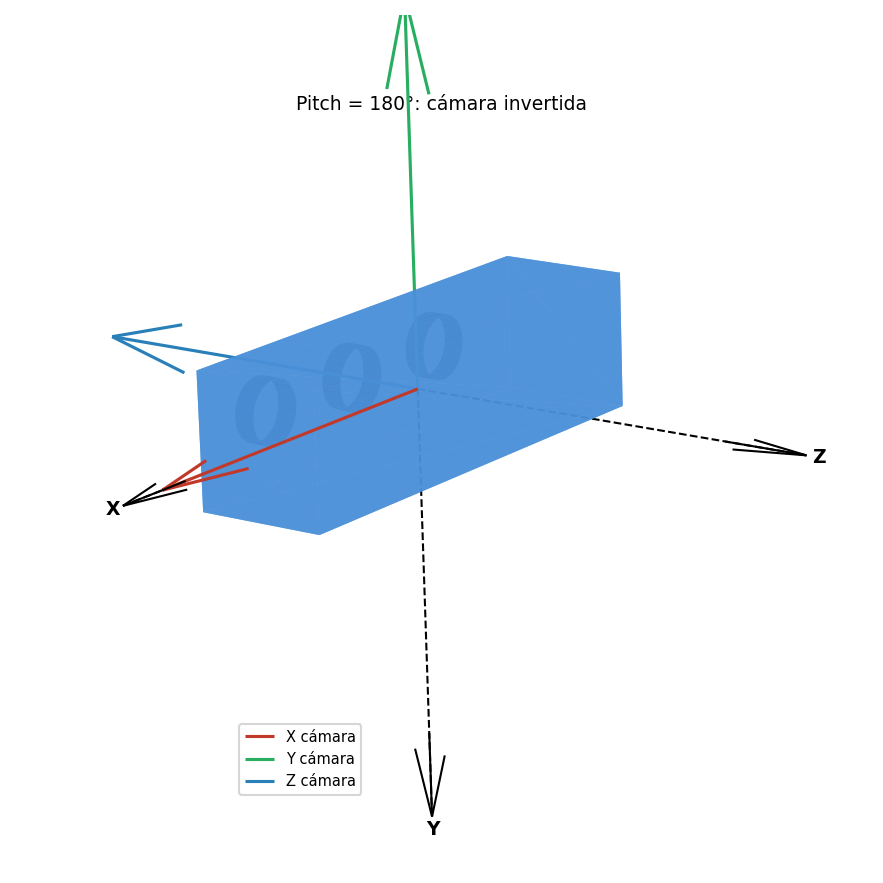
\includegraphics[width=\textwidth]{_Imagenes/local_mapper/pitch_180.png}
    \subcaption{Caso degenerado: pitch $= 180°$, $\hat{\mathbf{a}} = (0,+1,0) = -\hat{\mathbf{b}}$. \\
                $\hat{\mathbf{a}}\times\hat{\mathbf{b}} = \mathbf{0}$:
                eje indeterminado, se adopta rotación de $180°$ alrededor de $\hat{x}$,
                $q = (0,\,1,\,0,\,0)$.}
    \label{fig:rot-min-antiparallel}
  \end{minipage}
  \caption{Casos límite en el cálculo de la rotación mínima entre dos vectores.
           A la izquierda, la cámara horizontal produce un cuaternión identidad
           (sin corrección). A la derecha, la situación antiparalela requiere
           tratamiento especial para evitar indeterminación del eje de rotación.}
  \label{fig:rot-min-cases}
\end{figure}

\subsubsection{Filtrado del acelerómetro}

La señal del acelerómetro contiene ruido de alta frecuencia y puede presentar
picos transitorios debidos a golpes o aceleraciones repentinas del usuario.
Se aplica un filtro de primer orden (IIR \textit{low-pass}) sobre cada componente
de la aceleración~\cite{oppenheim1999dsp}, según la ecuación~\ref{eq:iir-filter}:
\begin{equation}
  \label{eq:iir-filter}
  \hat{a}_k = \alpha \cdot a_k + (1 - \alpha) \cdot \hat{a}_{k-1}
\end{equation}
donde $\alpha$ es el coeficiente de suavizado. Este filtro es la versión
discreta de un filtro paso bajos de primer orden continuo con función de
transferencia $H(s) = \omega_c / (s + \omega_c)$, donde
$\omega_c = 2\pi f_c$. Al discretizarlo por el método de Euler hacia
adelante con paso $T_s = 1/f_s$, la constante de tiempo discreta resulta en
la ecuación~\ref{eq:alpha}:

\begin{equation}
  \label{eq:alpha}
  \alpha = \frac{2\pi f_c}{2\pi f_c + f_s}
\end{equation}

La frecuencia de muestreo del IMU del D435i es $f_s = 200\,\text{Hz}$,
valor indicado en la hoja de datos del fabricante~\cite{RS-D400} y verificado
experimentalmente midiendo el tópico ROS correspondiente (200 mensajes por
segundo, tamaño medio de mensaje de $0{,}34\,\text{KB}$, ancho de banda
total de $68{,}3\,\text{KB/s}$). La frecuencia de corte $f_c = 5\,\text{Hz}$
es un parámetro de diseño que responde a dos criterios. Por un lado, la
marcha humana genera variaciones de inclinación a la frecuencia del paso
(típicamente $1{,}5$--$2\,\text{Hz}$)~\cite{menz2003acceleration}, por otro,
los movimientos voluntarios de la cabeza del usuario (asentir, girar para
orientarse) ocurren en ese mismo rango. Eligiendo $f_c = 5\,\text{Hz}$, la
frecuencia de corte supera en al menos $2{,}5\times$ la frecuencia máxima
de ambos fenómenos, garantizando que el filtro no introduzca desfase
perceptible en las señales de interés mientras atenúa el ruido mecánico de
alta frecuencia. Con estos
valores se obtiene $\alpha \approx 0{,}136$. La sintonización definitiva de
este parámetro queda sujeta a validación experimental con el dispositivo real.

Adicionalmente, se descartan las muestras cuya norma supera $2{,}5\,g$,
criterio que identifica golpes o perturbaciones mecánicas fuertes.

\subsection{Arquitectura}

El avance del alineador de gravedad introduce dos nuevas clases:

\begin{itemize}
  \item \texttt{ImuFilter}: encapsula el filtrado de la señal del
        acelerómetro (rechazo de outliers y filtro IIR low-pass). Recibe
        muestras crudas del acelerómetro y expone la aceleración filtrada
        en tres componentes.
  \item \texttt{GravityAligner}: calcula la rotación de corrección
        gravitacional a partir del vector de aceleración filtrado y la
        aplica a los puntos 3D de la nube. No tiene dependencias de ROS.
\end{itemize}

El nodo \texttt{depth\_projection\_node} incorpora una suscripción al
topic \texttt{imu} (remapeado desde \texttt{/camera/camera/imu}), pasa
cada muestra al \texttt{ImuFilter}, y utiliza el \texttt{GravityAligner}
al procesar cada frame de profundidad.

\subsection{Método de alineación}

El procedimiento completo para cada frame de profundidad es el siguiente:

\begin{enumerate}
  \item Se retroproyecta la imagen de profundidad a puntos 3D en el frame
        óptico (\texttt{camera\_depth\_optical\_frame}).
  \item Cada muestra del IMU actualiza el \texttt{ImuFilter}, que expone la
        aceleración filtrada $(\hat{a}_x,\, \hat{a}_y,\, \hat{a}_z)$.
  \item A partir de esa aceleración se calcula el cuaternión de rotación $q$
        que lleva el vector medido al eje ``abajo'' canónico $(0, -1, 0)$, y
        se publica como transformación TF dinámica
        \texttt{gravity\_aligned\_frame} $\to$ \texttt{camera\_depth\_optical\_frame}.
  \item La nube alineada se publica con los puntos \emph{sin rotar} en el frame
        \texttt{camera\_depth\_optical\_frame}. La corrección gravitacional
        queda codificada en la TF: cualquier consumidor (RViz, otro nodo) que
        solicite los puntos en \texttt{gravity\_aligned\_frame} obtiene los
        datos ya corregidos, sin necesidad de que el nodo aplique la rotación
        explícitamente punto a punto.
  \item La nube cruda se publica también sin rotar, pero en
        \texttt{gravity\_aligned\_frame} (fixed frame en RViz), de modo que
        se visualiza tal como la mide la cámara y oscila al inclinar el
        dispositivo.
\end{enumerate}

La separación entre el cálculo del cuaternión y la aplicación de la rotación
permite desacoplar ambas responsabilidades: el nodo se limita a mantener la
TF actualizada a la frecuencia del IMU, y los consumidores de la nube
alineada aplican la transformación cuando la necesitan mediante \texttt{tf2}.

\subsection{Implementación}

\paragraph{GravityAligner} La clase no depende de ROS: recibe flotantes y
retorna flotantes, lo que facilita su prueba unitaria sin necesidad de levantar
un nodo. El método \texttt{estimateOrientation(ax, ay, az)} implementa la
fórmula del cuaternión de rotación mínima descrita en la sección anterior.
El método \texttt{alignToGravity(px, py, pz, ax, ay, az)} combina ambas
operaciones en una sola llamada, útil desde el callback del nodo.

\paragraph{ImuFilter} Implementa el filtro IIR de primer orden con los
coeficientes mencionados ($\alpha = 0{,}136$). Incluye detección de dinámica
activa: cuando la norma de la aceleración filtrada se aleja más de
$0{,}5\,\text{m/s}^2$ de $1g$, se activa un flag \texttt{isDynamic()} que
las etapas superiores pueden consultar para inhibir la actualización de la
estimación.

\paragraph{Nodo} La suscripción al IMU usa \texttt{SensorDataQoS} (best
effort, alta frecuencia), coherente con los demás topics del sensor. Si el
IMU no ha llegado al momento de procesar el primer frame de profundidad, el
nodo emite un \texttt{WARN} y publica la nube alineada igual a la cruda (el
\texttt{ImuFilter} se inicializa con $(0, -g, 0)$, correspondiente a la
posición horizontal, lo que produce una TF identidad).

{\large\textcolor{red}{TO DO : Realizar medición/experimento}}

\subsection{Experimentos y mediciones propuestos}

Para validar el comportamiento del componente se proponen los siguientes
experimentos:

\begin{enumerate}
  \item \textbf{Cámara horizontal sobre superficie plana:} apoyar la cámara
        sobre una mesa nivelada y verificar en RViz que la nube alineada
        muestra el suelo como un plano horizontal (puntos con $y \approx$ cte),
        mientras que la nube cruda puede presentar inclinación.

  \item \textbf{Inclinación conocida:} inclinar la cámara un ángulo medido
        (por ejemplo $15°$ hacia abajo) y verificar que la nube alineada
        corrige esa inclinación. El ángulo de corrección puede calcularse a
        partir de la aceleración medida y compararse con el ángulo físico.

  \item \textbf{Estabilidad ante vibración:} someter el sensor a vibraciones
        suaves (mano sostenida) y verificar que la estimación de orientación
        no oscila significativamente gracias al filtro low-pass.

  \item \textbf{Comparación cruda vs. alineada en RViz:} captura de pantalla
        mostrando ambas nubes simultaneamente (transparente la cruda, opaca
        la alineada) junto con la imagen de color de referencia. La figura
        debe evidenciar la corrección del eje vertical.
\end{enumerate}
\iffalse
\begin{figure}[ht]
    \centering
    \includegraphics[width=0.95\textwidth]{_Imagenes/mapeo/rviz_aligned_cloud.png}
    \caption{Comparación en RViz de la nube cruda (semitransparente) y la nube
    alineada a gravedad (opaca) junto con la imagen de color de
    referencia. Se observa la corrección del eje vertical introducida
    por el componente \texttt{GravityAligner}.}
    \label{fig:rviz-aligned-cloud}
\end{figure}
\fi
